\documentclass{article}

\usepackage{kotex}
\usepackage{fancyhdr}
\usepackage{extramarks}
\usepackage{amsmath}
\usepackage{amsthm}
\usepackage{amsfonts}
\usepackage{amssymb}
\usepackage{tikz}
\usepackage[plain]{algorithm}
\usepackage{algpseudocode}

\usetikzlibrary{automata,positioning}

%
% Basic Document Settings
%

\topmargin=-0.45in
\evensidemargin=0in
\oddsidemargin=0in
\textwidth=6.5in
\textheight=9.0in
\headsep=0.25in

\linespread{1.1}

\pagestyle{fancy}
\lhead{\hmwkAuthorName}
\chead{\hmwkClass\ (\hmwkClassInstructor): \hmwkTitle}
\rhead{\firstxmark}
\lfoot{\lastxmark}
\cfoot{\thepage}

\renewcommand\headrulewidth{0.4pt}
\renewcommand\footrulewidth{0.4pt}

\setlength\parindent{0pt}

\newcommand\numberthis{\addtocounter{equation}{1}\tag{\theequation}}

%
% Create Problem Sections
%

\newcommand{\enterProblemHeader}[1]{
    \nobreak\extramarks{}{Problem \arabic{#1} continued on next page\ldots}\nobreak{}
    \nobreak\extramarks{Problem \arabic{#1} (continued)}{Problem \arabic{#1} continued on next page\ldots}\nobreak{}
}

\newcommand{\exitProblemHeader}[1]{
    \nobreak\extramarks{Problem \arabic{#1} (continued)}{Problem \arabic{#1} continued on next page\ldots}\nobreak{}
    \stepcounter{#1}
    \nobreak\extramarks{Problem \arabic{#1}}{}\nobreak{}
}

\setcounter{secnumdepth}{0}
\newcounter{partCounter}
\newcounter{homeworkProblemCounter}
\setcounter{homeworkProblemCounter}{1}
\nobreak\extramarks{Problem \arabic{homeworkProblemCounter}}{}\nobreak{}

%
% Homework Problem Environment
%
% This environment takes an optional argument. When given, it will adjust the
% problem counter. This is useful for when the problems given for your
% assignment aren't sequential. See the last 3 problems of this template for an
% example.
%
\newenvironment{homeworkProblem}[1][-1]{
    \ifnum#1>0
        \setcounter{homeworkProblemCounter}{#1}
    \fi
    \section{Problem \arabic{homeworkProblemCounter}}
    \setcounter{partCounter}{1}
    \enterProblemHeader{homeworkProblemCounter}
}{
    \exitProblemHeader{homeworkProblemCounter}
}

%
% Homework Details
%   - Title
%   - Due date
%   - Class
%   - Section/Time
%   - Instructor
%   - Author
%

\newcommand{\hmwkTitle}{Homework\ \#5}
\newcommand{\hmwkDueDate}{November 29, 2016}
\newcommand{\hmwkClass}{CS300}
\newcommand{\hmwkClassInstructor}{Prof. Sunghee Choi}
\newcommand{\hmwkAuthorName}{Ohjun Kwon}

%
% Title Page
%

\title{
    \vspace{2in}
    \textmd{\textbf{\hmwkClass:\ \hmwkTitle}}\\
    \normalsize\vspace{0.1in}\small{Due\ on\ \hmwkDueDate\ at 10:30am}\\
    \vspace{0.1in}\large{\textit{\hmwkClassInstructor}}
    \vspace{3in}
}

\author{\textbf{20160051 \hmwkAuthorName}}
\date{}

\renewcommand{\part}{\textbf{\large Part \Alph{partCounter}}\stepcounter{partCounter}\\}

%
% Various Helper Commands
%

% Useful for algorithms
\newcommand{\alg}[1]{\textsc{\bfseries \footnotesize #1}}

% For derivatives
\newcommand{\deriv}[1]{\frac{\mathrm{d}}{\mathrm{d}x} (#1)}

% For partial derivatives
\newcommand{\pderiv}[2]{\frac{\partial}{\partial #1} (#2)}

% Integral dx
\newcommand{\dx}{\mathrm{d}x}

% Alias for the Solution section header
\newcommand{\solution}{\textbf{\large Solution}}

% Probability commands: Expectation, Variance, Covariance, Bias
\newcommand{\E}{\mathrm{E}}
\newcommand{\Var}{\mathrm{Var}}
\newcommand{\Cov}{\mathrm{Cov}}
\newcommand{\Bias}{\mathrm{Bias}}

\begin{document}

\maketitle

\pagebreak
\begin{homeworkProblem}
    수업시간에 제시되었던 \alg{BFS} 코드를 보자.
    \begin{algorithm}[!ht]
        \begin{algorithmic}[1]
            \Function{BFS}{$G,s$}
                \State \Call{Enqueue}{$Q,s$}
                \While{$Q\neq \varnothing$}
                    \State $u\gets $ \Call{Dequeue}{$Q$}
                    \For{each $v\in Adj[u]$}
                        \If{$d[v]=\infty$}
                            \State $d[v]\gets d[u]+1$
                            \State \Call{Enqueue}{$Q,v$}
                        \EndIf
                    \EndFor
                \EndWhile
            \EndFunction
        \end{algorithmic}
    \end{algorithm}
    이러한 \alg{BFS} 코드는 $Adj[i]$를 보면 알 수 있듯이 인접리스트를 이용하여
    그래프의 간선에 대한 정보를 알아내고 있다. 하지만, 우리의 경우에는 인접행렬을
    이용하여 알고리즘을 다루고 싶은 경우이다. 이도 \alg{BFS}\와 비슷한 형식으로
    작성하면 된다. $Adj[u]$가 들어가있는 부분만 바꾸어주면 된다. 쉽게 생각하면
    인접리스트를 이용한 \alg{BFS}의 시간복잡도인 $O(V+E)$에서 간선을 찾는데 걸리는
    시간이 $E$가 아니라 $V^2$임에서 착안하여 $O(V^2)$이 됨을 대략적으로 알 수 있지만,
    직접적으로 알고리즘을 작성하여 시간복잡도가 어떻게 되는지 알아보자.
    \begin{algorithm}[!ht]
        \begin{algorithmic}[1]
            \Function{BFS'}{$G,s$}
                \State \Call{Enqueue}{$Q,s$}
                \While{$Q\neq \varnothing$}
                    \State $u\gets $ \Call{Dequeue}{$Q$}
                    \For{$i\gets 1$ to $|V|$}
                        \If{$G[u,i]=1$}
                            \If{$d[i]=\infty$}
                                \State $d[i]\gets d[u]+1$
                                \State \Call{Enqueue}{$Q,i$}
                            \EndIf
                        \EndIf
                    \EndFor
                \EndWhile
            \EndFunction
        \end{algorithmic}
    \end{algorithm}
    \alg{BFS'}의 의사코드를 보면 $Adj[u]$가 있을 부분에 인접행렬의 한 행을 전부
    검사하여 간선으로 연결되어있는 정점을 찾는 코드가 보인다. 한 정점에 대하여
    총 $|V|$개의 정점에 대하여 검사를 하게 되므로 $O(V)$이고, 이를 각 정점에
    대하여 모두 한 번씩은 연산하기 때문에 총 시간복잡도는 $O(V^2)$이 된다.
\end{homeworkProblem}

\begin{homeworkProblem}
    우리가 보이고 싶은 것은 그래프의 모든 cut에 대해 교차하는 유일한 light edge를
    가질 때, 그 그래프는 유일한 최소신장트리를 가짐을 보이는 것이다. 이를 증명하기
    위해 귀류법을 이용하자. 먼저 서로 다른 두 개의 MST $M$, $S$가 있다고 가정하고,
    사실은 이 둘이 같음을 보이면 증명이 완료된다. 두 트리가 같다는 것은 $M$에 속한
    임의의 간선이 $S$에 속하고 $S$에 속한 임의의 간선이 $M$에 속함을 보여 트리에
    포함된 모든 간선이 같음을 보이는 방법으로 할 수 있다.

    먼저, $M$에 속한 임의의 간선 $(u,v)$를 생각하자. 이 간선을 지운다면 최소신장트리인
    $M$은 두 부분으로 \textbf{절단}될 것이다. 이 절단을 $(A, V-A)$라고 하고(이 절단에서
    교차하는 간선은 $(u,v)$로 유일하므로 $(u,v)$는 $M$의 절단 $(A,V-A)$에 교차하는
    light edge이다), 동일한 정점 $V$로 이루어진 최소신장트리 $S$에서 이 절단에 대해 생각해보자.
    트리를 $(A,V-A)$와 같이 절단할 때 교차하는 light edge는 가정에 의해 유일하기
    때문에 간선 $(u,v)$는 트리 $S$에도 포함된다. 반대방향으로도 동일한 방법으로
    ($M$과 $S$의 위치를 바꾸면) 증명될 수 있다. $\therefore$ $M$과 $S$는 동일한 트리이다.

    이 명제의 역은 ``유일한 최소신장트리를 가지는 그래프이면, 그래프의 모든 cut에 대해 교차하는
    유일한 light edge를 가진다''이다. 이 명제에 대한 반례는 아래 그림~\ref{fig:21}\과 같다.
    \begin{figure}[!htb]
        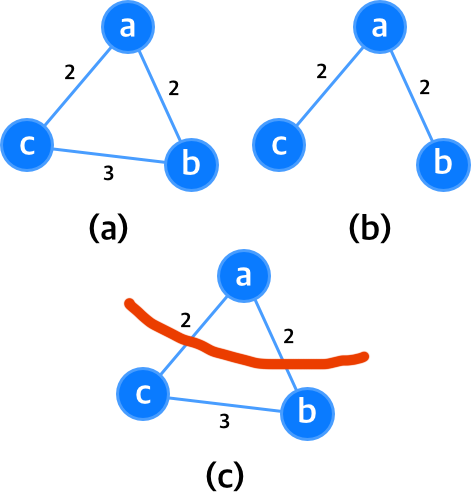
\includegraphics[height=0.3\textheight]{2-1}
        \centering
        \caption{반례}
        \label{fig:21}
    \end{figure}
    그림~\ref{fig:21}~(a)와 같은 그래프가 반례가 된다. 그림~\ref{fig:21}~(a)의 최소신장트리는
    그림~\ref{fig:21}~(b)로 유일하다. 하지만 그림~\ref{fig:21}~(a)의 절단 중 하나인
    그림~\ref{fig:21}~(c)와 교차하는 light edge는 $(a,b)$, $(a,c)$로 유일하지 않다.
\end{homeworkProblem}

\begin{homeworkProblem}
    원하는 식은 곱으로 표현되어 있기 때문에 우리가 가지고 있는 기술인 그래프 상에서의
    최단 경로를 구하는 방법을 사용하지 못한다. 주어진 식~\ref{eq:31}\을 덧셈 꼴로
    변형하기 위해서 양변에 로그를 취해주자.
    \begin{align*}
        R[i_1,i_2]\cdot R[i_2,i_3]\cdot \dots R[i_{k-1},i_k]\cdot R[i_k,i_1] &> 1 \label{eq:31} \numberthis \\
        \lg\left\{R[i_1,i_2]\cdot R[i_2,i_3]\dots R[i_{k-1},i_k]\cdot R[i_k,i_1]\right\} &> \lg 1 \\
        \lg R[i_1,i_2] + \lg R[i_2,i_3] + \dots + \lg R[i_k,i_1] &> 0 \label{eq:32} \numberthis
    \end{align*}
    식~\ref{eq:32}\이 얻어졌는데, 여기서 양변에 $-1$을 곱해주면 식~\ref{eq:33}\과 같은 꼴이 만들어진다.
    각 통화가 정점을 의미하고 환율이 간선을 의미하는 방향 그래프를 생각해보자.
    각 $-\lg R[i_a, i_b]$\를 두 노드 $a$와 $b$를 잇는 간선의 가중치라고 하면 부등식~\ref{eq:31}\을 변형하여
    얻은 동치인 식~\ref{eq:33}\은 그래프에서 음의 가중치를 갖는 순환을 의미하게 되고, 주어진 문제는
    그래프에서 음의 가중치를 갖는 순환을 찾는 문제로 환원된다.
    \begin{align*}
        -\lg R[i_1,i_2] + -\lg R[i_2,i_3] + \dots + -\lg R[i_k,i_1] < 0 \label{eq:33} \numberthis
    \end{align*}
    벨만-포드 알고리즘을 이용하여 방향 그래프에서 음의 가중치를 갖는 순환을 가지는지 여부를 찾는
    알고리즘을 우리는 수업시간에 작성하였으므로 자세한 설명은 생략하고, 벨만-포드 알고리즘을 이용하여
    그래프가 음의 가중치를 갖는 순환을 갖는지 여부만 판별하는 것이 아니라 그 순환을 출력해야 하므로
    수업시간에 작성했던 벨만-포드 알고리즘에 약간의 수정을 가하도록 하자. (python 2로 작성된 작동하는
    알고리즘(prob3.py)은 별도의 페이지로 첨부되어있다. cf) 0-based index로 짜여진 소스이다.)

    가장 먼저 \alg{bellford}\는 정상적인 벨만-포드 알고리즘의 알고리즘에서 음의 가중치를 갖는 순환
    검출 부분에 삼각부등식이 성립하지 않은 곳을 저장하도록 하였다. 모든 relaxation step이 끝난 이후에도
    $d$ 값이 변하는 이유는 바로 음의 가중치를 갖는 순환이 있기 때문에 $d$ 값이 계속 작아질 수 있는 것이다.
    이렇게 확인된 정점에서 바로 직전에 방문했던 정점인 $p$를 따라가면 순환을 검출할 수 있게 된다.
    하지만, 이 순서대로 출력하면 간선의 방향의 반대방향으로 출력되게 되므로 스택에 저장 후 하나씩 pop하면서
    출력하면 음의 가중치를 갖는 경로를 검출할 수 있게 된다.

    하지만, 벨만-포드 알고리즘은 전체를 탐색하는 것이 아니고 하나의 source에서 나아가는 경로를 탐색하는
    알고리즘이므로 모든 정점에 대해 각각 음의 가중치를 갖는 경로를 찾을 수 있는지 검사하여야 한다.
    \alg{bellford}의 시간복잡도는 정상적인 원래의 벨만-포드 알고리즘 뒤에 경로를 추적하는 루틴을 넣었으므로
    $O(V^3+V)=O(V^3)$인데 이를 각 정점마다 실행하게 되므로 \alg{findCycle}의 시간복잡도는 총 $O(V^4)$가
    된다.

    \alg{bellford}를 모든 정점에 대해서 실행시켜야 하는 이유는 그림~\ref{fig:31} 같은 그래프에서 $0$이나 $1$을
    source로 선택하는 경우 모든 정점과의 $d$가 $\infty$이기 때문에 경로를 찾을 수 없기 떄문이다. 약간의 편법을
    이용하면 모든 정점에 대하여 확인해보지 않아도 알 수 있는데, $\infty$의 값 대신 매우 큰 자연수 값을 주게 되면
    $\infty$의 역할도 하는 동시에 $d$ 값이 감소할 수 있어 아무 정점이나 source로 선택하여 \alg{bellford}를
    실행하면 음의 가중치를 갖는 순환을 찾을 수 있다. 이렇게 되면 $O(V^3)$만에 찾을 수 있게 되는 것이다.
    \begin{figure}[!htb]
        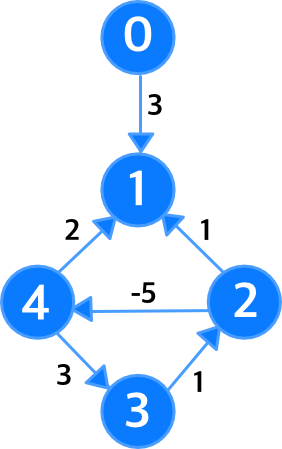
\includegraphics[height=0.3\textheight]{3-1}
        \centering
        \caption{예시}
        \label{fig:31}
    \end{figure}
\end{homeworkProblem}
\end{document}
